\section{实验结果}

\subsection{数据的预处理与函数的设置}

\subsubsection{数据的预处理}
编写python程序,将CHI软件保存的.txt文件识别并存储到python中自定义的数据结构 Segment() 与 CyclicVoltammetry() 中,方便之后的调用。

\subsubsection{函数的设置}

使用python编写一些数据处理中必要的函数,以下是它们的简要介绍:
\begin{itemize}
    \item merge\_df() 将正反的扫描数据首尾相连,形成闭合的CV曲线;
    \item float\_to\_sci() 将浮点数转化为 \LaTeX 格式的科学计数法字符串;
    \item find\_cross\_point()找出两条曲线在的交点坐标;
    \item save\_data() 保存数据至csv格式。
\end{itemize}

\subsection{氮气饱和下测定不同扫速的 CV 曲线}

在 $\mathrm{N}_2$ 饱和下,测定不同扫速 $(0.5 \mathrm{~V} / \mathrm{s} $、$ 0.2 \mathrm{~V} / \mathrm{s} $、$ 0.1 \mathrm{~V} / \mathrm{s}$ 的 $0.05 \mathrm{~mol} / \mathrm{L}$ 硫酸溶液的 CV 曲线,取 Segments 4、5 的数据,使用python matplotlab绘图,得到图 \ref{fig:1}。

\begin{figure}[htbp]
    \centering
    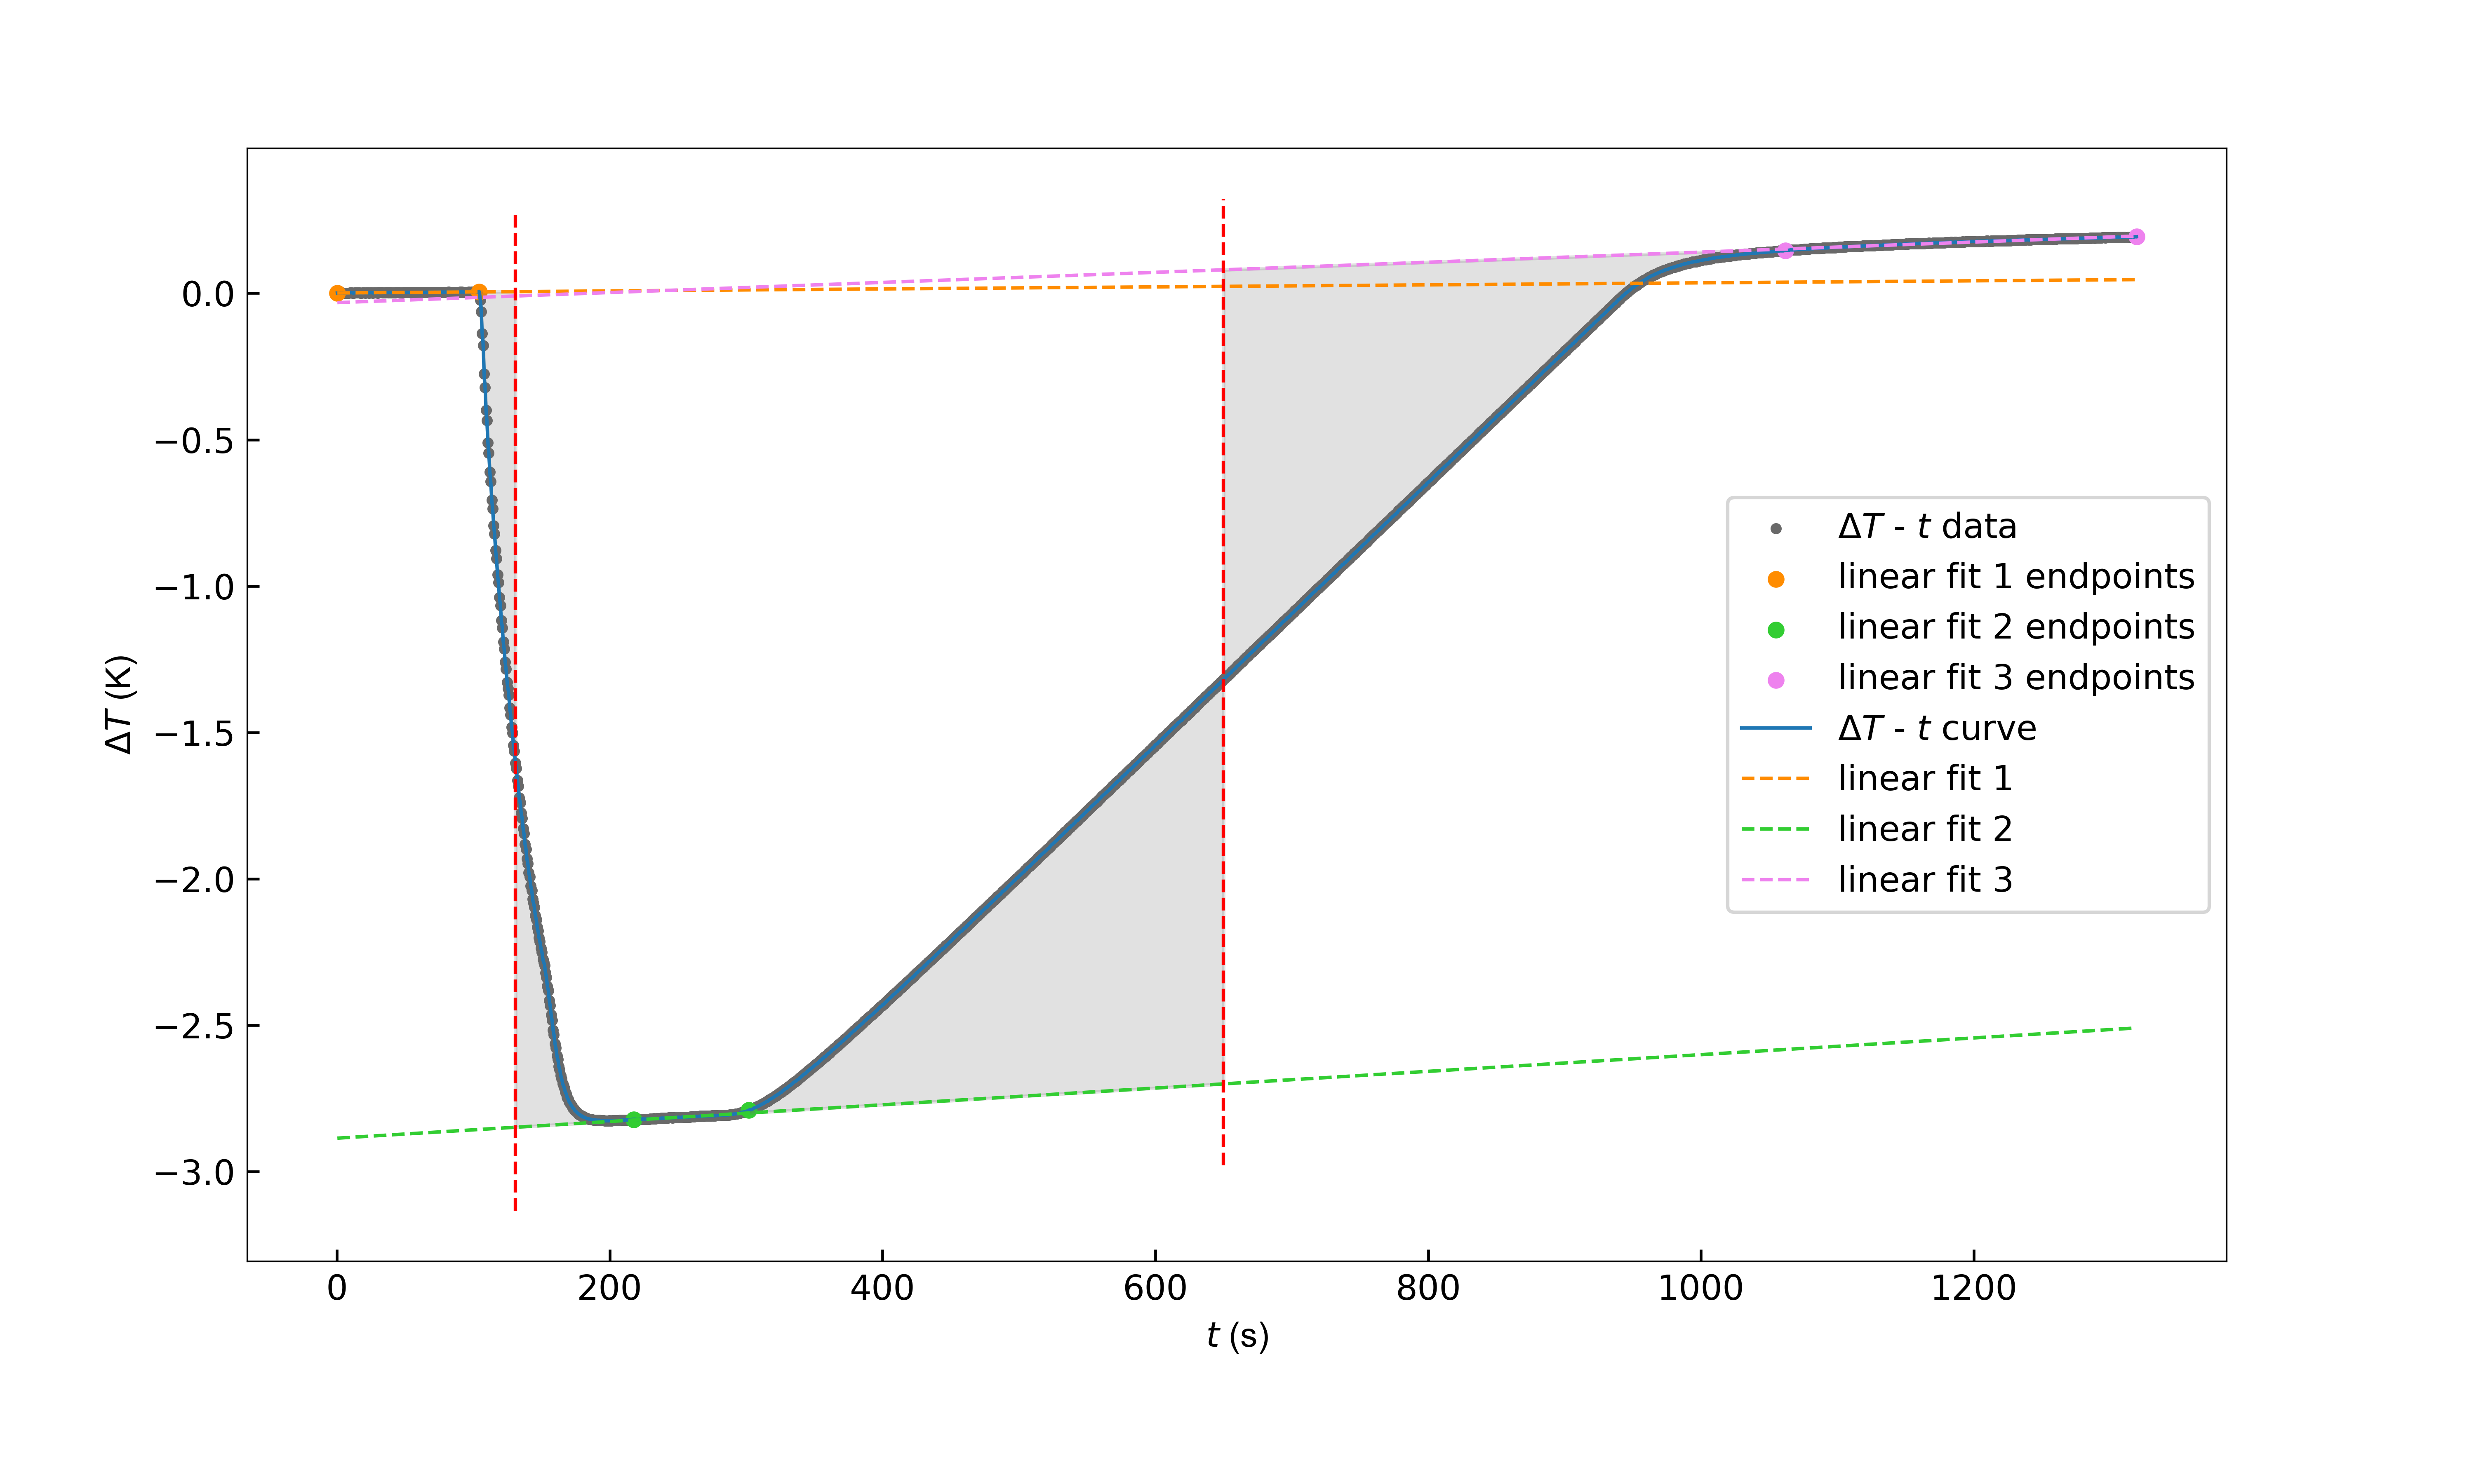
\includegraphics[width=.75\textwidth]{figures2/1.png}
    \bicaption{不同扫速 0.05 mol/L 硫酸溶液的 CV 曲线图}{CV Curves of 0.05 mol/L Sulfuric Acid Solution at Different Scan Rates}
    \label{fig:1}
\end{figure}

根据图 \ref{fig:1},观察到:
\begin{enumerate}
    \item 在氢区(图的左侧两个峰),我们观察到较好的对称性,这表明反应具有良好的可逆性。具体而言,这意味着氢的吸附与脱附过程具有较好的可逆性。
    \item 相比之下,氧区(图的右侧)的对称性较差,仅呈现还原峰而没有对应的氧化峰。这表明在这一区域发生了不可逆的氧还原反应。
    \item 峰电势的大小对扫描速率并不敏感,而电流峰值却与扫描速率呈正相关关系。这符合循环伏安法的基本原理:根据 Randles-Ševčík 方程,峰电流 $i_p$ 满足:
    $$
    i_p=0.4463 n F A C \sqrt{\frac{n F v D}{R T}} \propto \sqrt{v}
    $$
    其中,$v$ 为扫描速度。
\end{enumerate}

\subsection{不同条件下铂电极表面的氧还原反应的 CV 曲线}

固定扫速为\SI{0.1}{V/s},测定不同条件下的铂电极表面的氧还原反应的 LSV 曲线,取Segment 10的数据,使用python matplotlab绘图,得到图 \ref{fig:2}。其中,$\ce{N2}+\neg$stirring 表示\ce{N2}饱和不搅拌;$\neg\ce{O2}+\neg$stirring 表示在饱和\ce{O2}的溶液中不继续通入\ce{O2},且不搅拌;$\ce{O2}+\neg$stirring 表示\ce{O2}饱和不搅拌;$\ce{O2}+$stirring 表示\ce{O2}饱和并搅拌。

\begin{figure}[htbp]
    \centering
    \includegraphics[width=.75\textwidth]{figures2/2.png}
    \bicaption{不同条件下Pt电极表面氧还原反应的 LSV 曲线}{LSV Curves of Oxygen Reduction Reaction on Pt Electrode under Different Conditions}
    \label{fig:2}
\end{figure}

从图 \ref{fig:2} 可以看出,在不同条件下,氧还原反应的线性扫描伏安 (LSV) 曲线走势大致相同。具体来说:

\begin{enumerate}
    \item 对于不涉及氧还原反应的部分(电势高于 $0.6 \mathrm{~V}$),不同搅拌速度下的 LSV 曲线基本重合。
    \item 在电势较低的氧还原电势区(电势低于 $0.6 \mathrm{~V}$),随着搅拌的增强,氧还原的峰电流 $i_p$ 增大,且 LSV 曲线的波动更为明显。这是因为在快速搅拌下,物质传输加快,铂电极附近消耗的 $\mathrm{O}_2$ 和 $\mathrm{H}^{+}$ 得到及时补充,导致氧还原的峰电流较大;同时,快速搅拌对铂电极附近溶液的扰动导致 $\mathrm{O}_2$ 和 $\mathrm{H}^{+}$ 浓度变化剧烈,从而使 LSV 曲线产生显著波动。
\end{enumerate}

在不搅拌时,分别比较\ce{N2}与\ce{O2}通气饱和的CV曲线,取Segment 9-10的数据,使用python matplotlab绘图,得到图 \ref{fig:3}。

\begin{figure}[htbp]
    \centering
    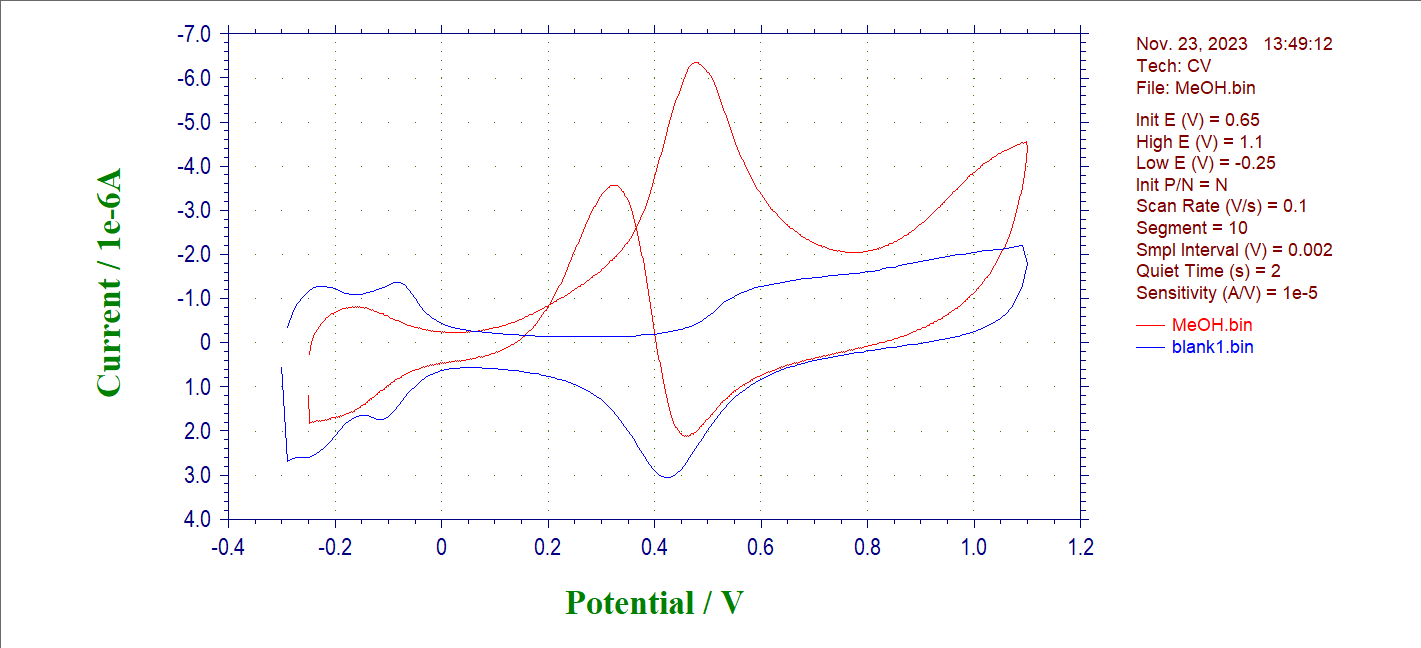
\includegraphics[width=.75\textwidth]{figures2/3.png}
    \bicaption{氮气与氧气饱和的硫酸溶液中的 CV 曲线}{CV curve in sulfuric acid solution saturated with nitrogen and oxygen}
    \label{fig:3}
\end{figure}

根据图 \ref{fig:3},使用 python 求出两条曲线各自的起始还原电位
\begin{align*}
    E_{red,1} &= \SI{0.627}{V}\\
    E_{red,2} &= \SI{0.600}{V}
\end{align*}
可以求得氧化过程中氧的过电势 $\eta_{\rm O}$
$$
\eta_{\rm O} = E_{red,1} - E_{red,2}=\SI{0.027}{V}
$$

过电势 $\eta_{\mathrm{O}}$ 的形成可能源于含氧物种在铂电极表面的吸附和氧化过程。在这一过程中,氧气的电化学反应在铂电极表面进行得较慢,导致电化学极化现象。这种极化使得在电势升高和降低过程中,氧气的起始氧化电位和起始还原电位出现不一致。


\subsection{铂电极表面的甲醇电化学氧化反应}

固定扫速为\SI{0.1}{V/s},测定硫酸溶液中铂电极表面甲醇电化学氧化与氮气饱和的 CV 曲线,取Segment 9-10的数据,使用python matplotlab绘图,得到图 \ref{fig:4}。

\begin{figure}[htbp]
    \centering
    \includegraphics[width=.75\textwidth]{figures2/4.png}
    \bicaption{硫酸溶液中甲醇氧化与氮气饱和的 CV 曲线}{CV curve of methanol oxidation and nitrogen saturation in sulfuric acid solution}
    \label{fig:4}
\end{figure}

根据图 \ref{fig:4},使用 python 求出甲醇的起始氧化电位为 \SI{0.026}{V}。

\subsection{铂电极的电化学活性面积}

利用氮气饱和的硫酸溶液中铂电极的 $\mathrm{CV}$ 曲线中氢原子脱附峰的电量求算铂电极的电化学活性面积。取三种不同扫描速度下的 $\mathrm{CV}$ 曲线 Segment 9-10 的实验数据,以双电层电位作为基线,使用 python 编写程序,对氢原子吸脱附峰峰面积进行积分,得到氢原子吸脱附峰的电量,结果如图 \ref{fig:5} 所示,图中红色虚线即为双电层电位基线,阴影为积分面积。

\begin{figure}[htbp]
    \centering
    \begin{subfigure}{0.49\textwidth}
        \centering
        \includegraphics[width=\linewidth]{figures2/5-1.png}
    \end{subfigure}
    \hfill
    \begin{subfigure}{0.49\textwidth}
        \centering
        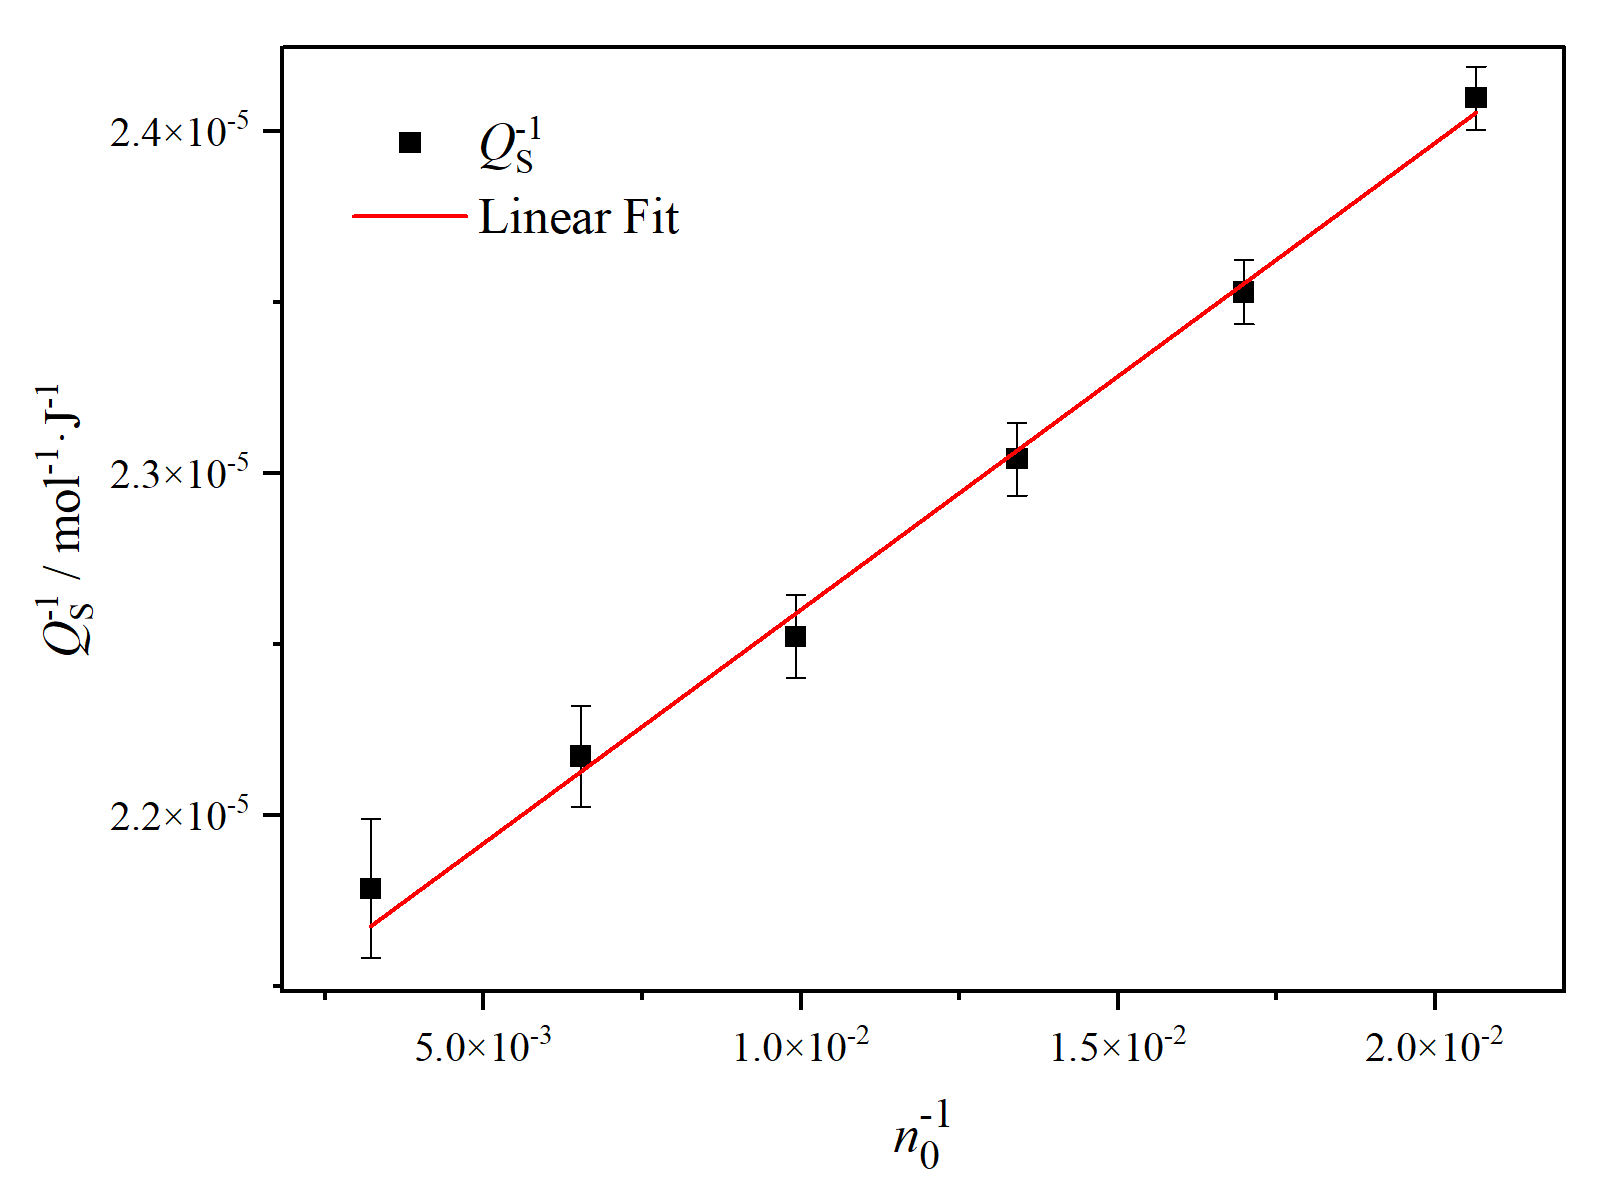
\includegraphics[width=\linewidth]{figures2/5-2.png}
    \end{subfigure}
    \vspace{1em} % Adjust the vertical spacing as needed
    \begin{subfigure}{0.49\textwidth}
        \centering
        \includegraphics[width=\linewidth]{figures2/5-3.png}
    \end{subfigure}
    \hfill
    \begin{subfigure}{0.49\textwidth}
        \centering
        \includegraphics[width=\linewidth]{figures2/5-4.png}
    \end{subfigure}
    \vspace{1em} % Adjust the vertical spacing as needed
    \begin{subfigure}{0.49\textwidth}
        \centering
        \includegraphics[width=\linewidth]{figures2/5-5.png}
    \end{subfigure}
    \hfill
    \begin{subfigure}{0.49\textwidth}
        \centering
        \includegraphics[width=\linewidth]{figures2/5-6.png}
    \end{subfigure}
    \bicaption{由铂电极 CV 曲线积分求氢原子吸脱附峰电量}{H absorp./desorp. peak electricity calculation by integrating the CV curve of Pt electrode}
    \label{fig:5}
\end{figure}

获知积分面积$S$后,可以求得在固定扫速时,氢的吸附/脱附量
\begin{equation}\label{eq:1}
    Q_{\mathrm{H},absorp./desorp.}=\int \frac{I}{v} \mathrm{~d} V= \frac{1}{v}\int I\mathrm{~d} V
\end{equation}
进一步地,可以求得铂电极的电化学活性面积\cite{pcl2002}为
\begin{equation}\label{eq:2}
    E S A=\frac{Q_{\mathrm{H},desorp.}}{2.10 ~\mu \mathrm{C} \cdot \mathrm{mm}^{-2}}
\end{equation}

根据图 \ref{fig:5} 中的计算结果,结合公式 \ref{eq:1} 与公式 \ref{eq:2},计算得到不同扫速时的铂电极的电化学活性面积$ESA$如表 \ref{tab:1}。

\begin{table}[htbp]
    \centering
    \bicaption{不同扫速时的铂电极电化学活性面积}{ESA of Platinum Electrode at Different Scan Rates}
    \begin{tabular}{ccccc}
    \toprule
        $v$/\si{V\cdot s^{-1}} & $S$/\si{V\cdot A} & $Q_{\mathrm{H},absorp./desorp.}$/\si{\mu C} & $ESA$/\si{mm^2} \\
        \midrule
        +0.1 & $4.85\times 10^{-7}$ & 4.85 & 2.31 \\
        -0.1 & $4.85\times 10^{-7}$ & 4.85 & 2.31 \\
        +0.2 & $8.46\times 10^{-7}$ & 4.23 & 2.02 \\
        -0.2 & $8.46\times 10^{-7}$ & 4.23 & 2.02 \\
        +0.5 & $1.89\times 10^{-6}$ & 3.79 & 1.81 \\
        -0.5 & $1.89\times 10^{-6}$ & 3.79 & 1.81 \\
        \bottomrule
    \end{tabular}
    \label{tab:1}
\end{table}

由表 \ref{tab:1} 可以发现,随着扫速的增加,铂电极的电化学活性面积在减少,这与氢气在铂电极表面吸附的动力学速率限制有关。

\subsection{直接甲醇燃料电池输出电压-输出功率曲线}

设定扫描速度为 $0.1 \mathrm{~V} \cdot \mathrm{s}^{-1}$,以 $\mathrm{N}_2$ 饱和的硫酸溶液中铂电极的 $\mathrm{CV}$ 曲线 Segment 4 的实验数据为背景,取电解质静止、$\mathrm{O}_2$ 饱和的硫酸溶液中铂电极的 $\mathrm{CV}$ 曲线第 Segment 10 的实验数据,扣除背景后,作为直接甲醇燃料电池 $\mathrm{Pt}$ 电极阴极 $\mathrm{O}_2$ 还原的 $\varphi-i$ 工作曲线;以 $\mathrm{N}_2$ 饱和的硫酸溶液中铂电极的 $\mathrm{CV}$ 曲线 Segment 5 的实验数据为背景,取硫酸溶液中铂电极表面 $\mathrm{MeOH}$ 电化学氧化反应的 $\mathrm{CV}$ 曲线 Segment 9 的实验数据,扣除背景后,作为直接甲醇燃料电池 $\mathrm{Pt}$ 电极阳极 $\mathrm{MeOH}$ 氧化的 $\varphi-i$ 工作曲线。使用 python 编程,绘制两条 $\varphi-i$ 曲线如图 \ref{fig:6} 所示。

\begin{figure}[htbp]
    \centering
    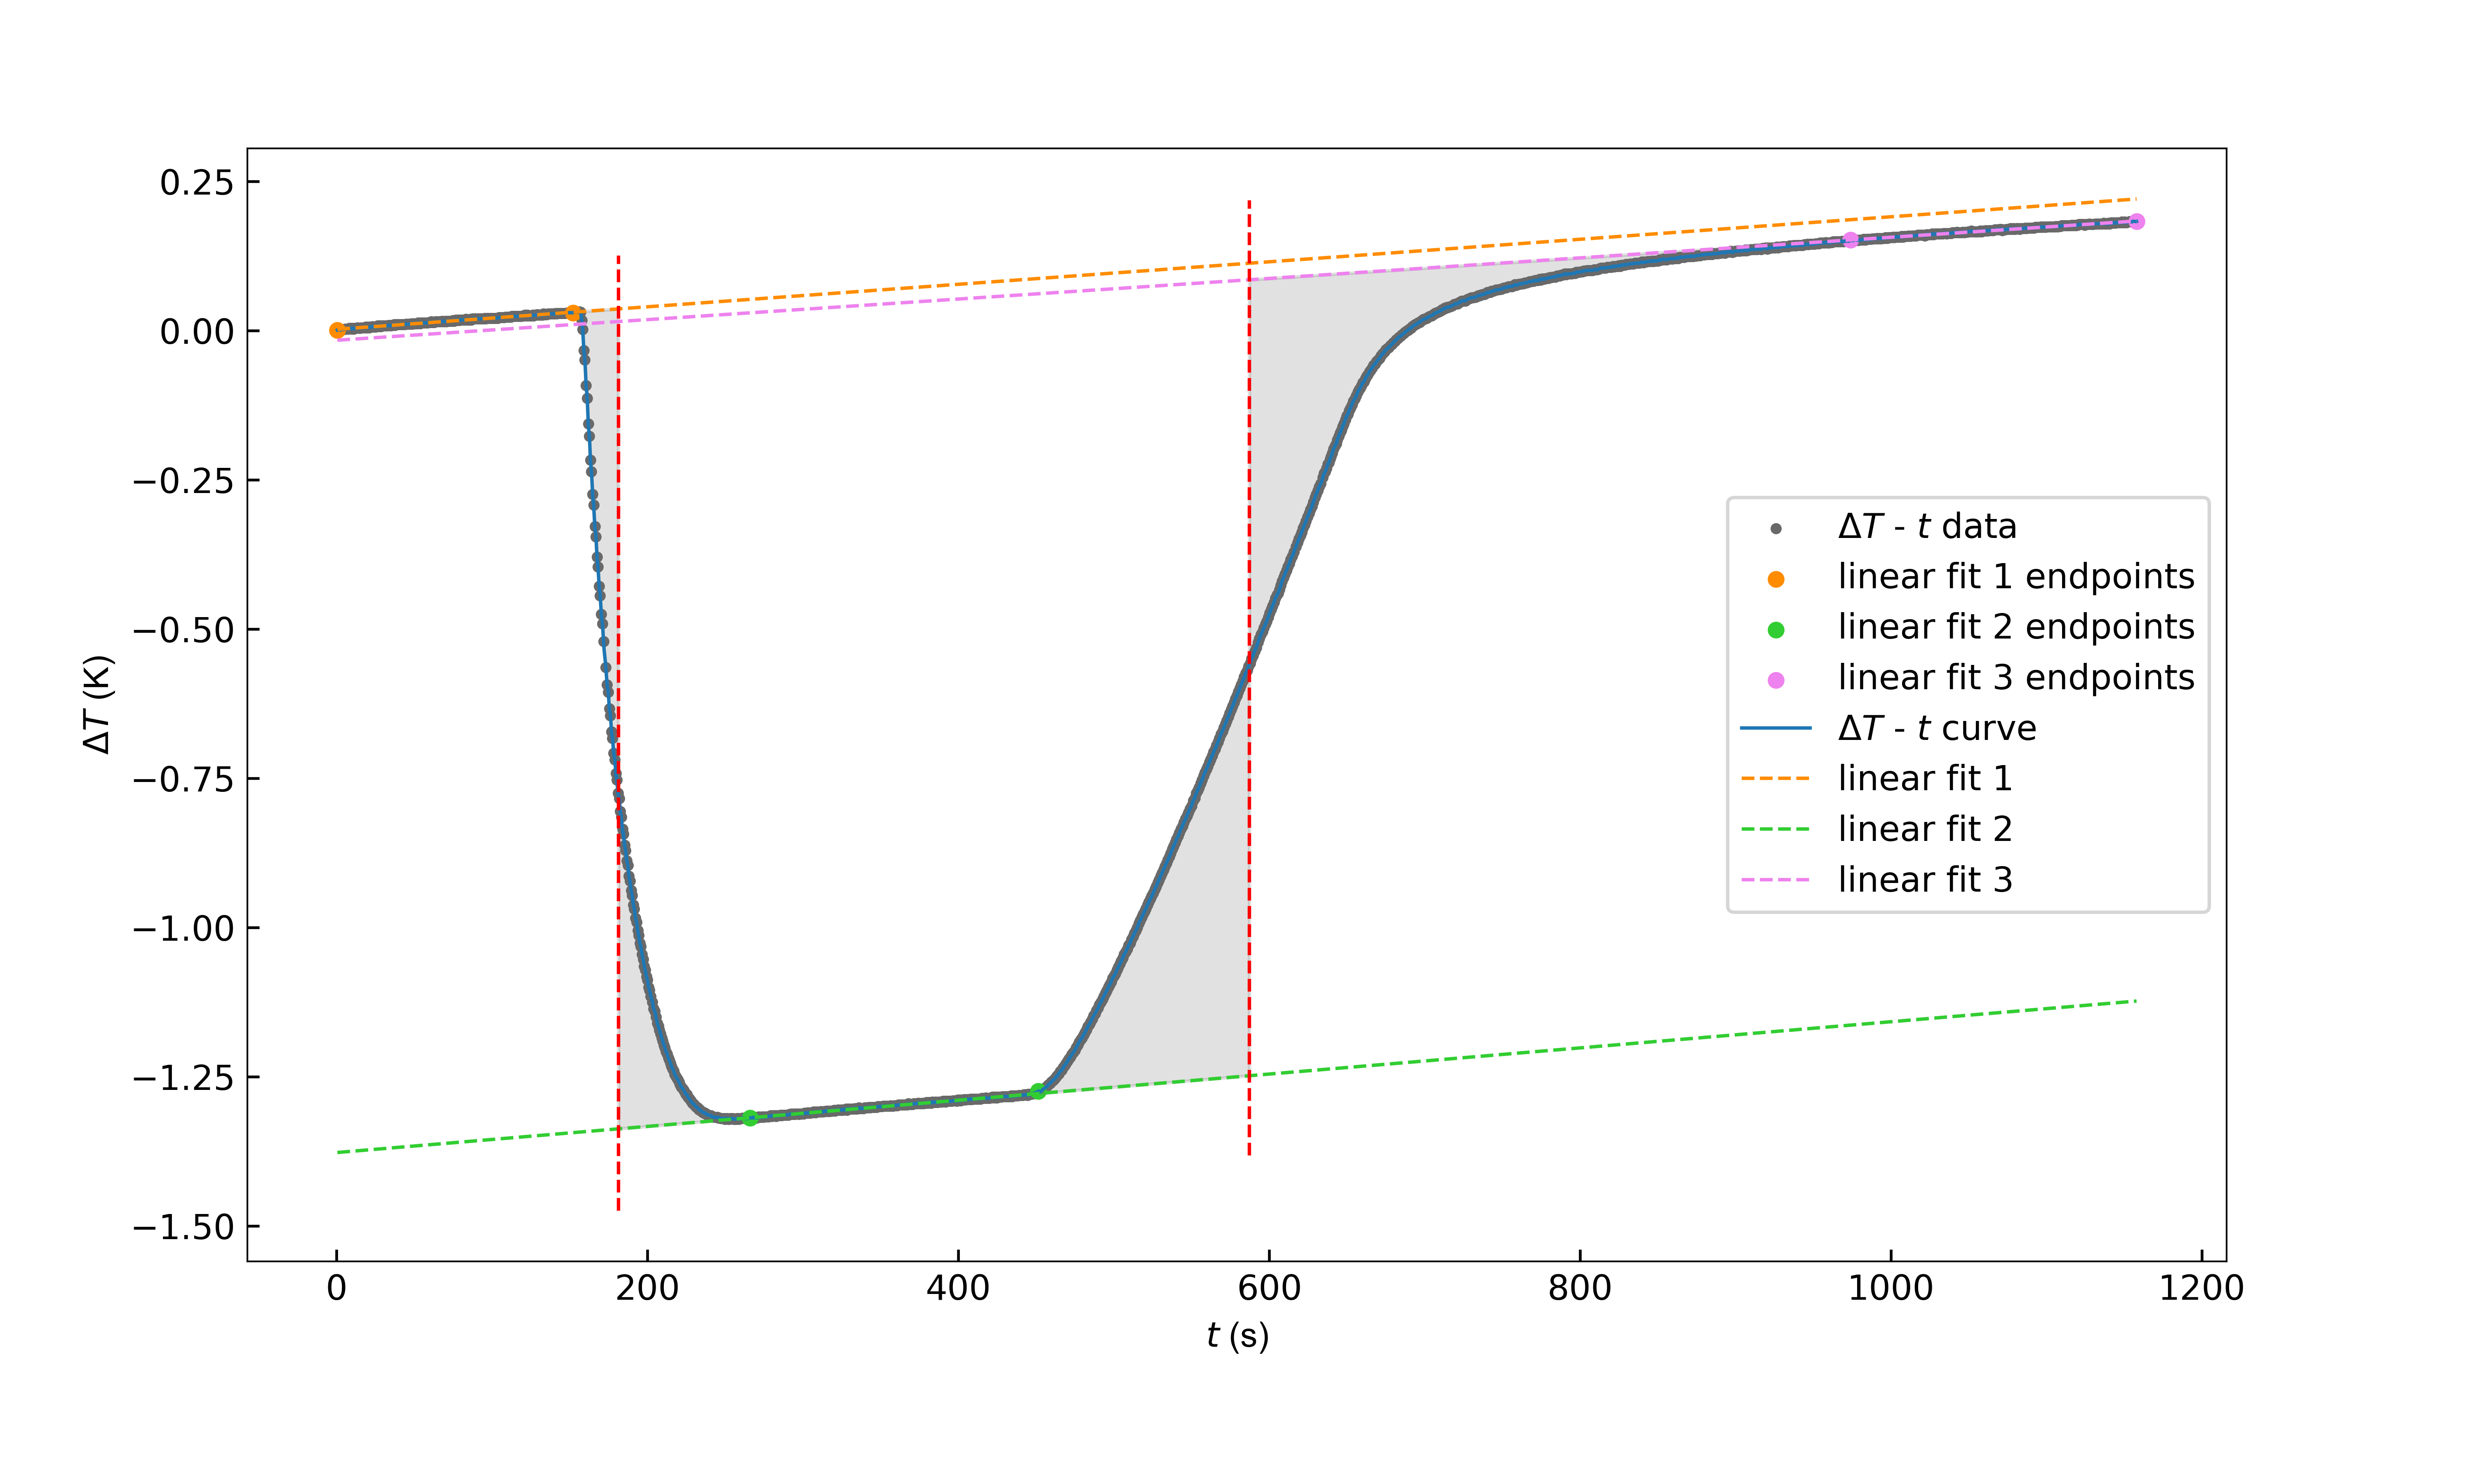
\includegraphics[width=.75\textwidth]{figures2/6.png}
    \bicaption{直接甲醇燃料电池阳极、阴极 $\varphi-i$ 工作曲线}{$6 \quad \varphi-i$ working curve of anode and cathode of direct methanol fuel cell}
    \label{fig:6}
\end{figure}

在直接甲醇燃料电池中,在一定的工作电流 $i$ 下,阳极(负极,甲醇氧化) 电势 $\varphi_a$ 低于阴极(正极,氧气还原)电势 $\varphi_c$ 。在图 \ref{fig:6} 中选取 $i$ 相同时 $\varphi_a<\varphi_c$ 的部分,使用 python 编程,作 1000 组平行于 $\varphi$ 轴的直线与两条曲线相交,读取交点坐标对应的电势 $\varphi_a $、$ \varphi_c$,计算两极电势差即为直接甲醇燃料电池的输出电压
\begin{equation}\label{eq:3}
    U=\varphi_c-\varphi_a
\end{equation}

根据公式 \eqref{eq:3},绘制直接甲醇燃料电池的$U-I$曲线,如图 \ref{fig:7}。

\begin{figure}[htbp]
    \centering
    \includegraphics[width=.75\textwidth]{figures2/7.png}
    \bicaption{直接甲醇燃料电池的$U-I$曲线}{$U-I$ Curve of Direct Methanol Fuel Cell}
    \label{fig:7}
\end{figure}

根据
$$
P=U i
$$

计算直接甲醇燃料电池的输出功率 $P$,绘制直接甲醇燃料电池的$U-P$曲线,如图 \ref{fig:8}。

\begin{figure}[htbp]
    \centering
    \includegraphics[width=.75\textwidth]{figures2/8.png}
    \bicaption{直接甲醇燃料电池的$U-P$曲线}{$U-P$ Curve of Direct Methanol Fuel Cell}
    \label{fig:8}
\end{figure}

根据图 \ref{fig:8} 可知,直接甲醇燃料电池的输出功率 $P$ 随输出电压 $U$ 的增大而先增大后减小,存在一个极大值。使用 python 求出曲线的顶点坐标,对应着 $U = \SI{0.173}{V}$、$P=3.73\times 10^{-7}\mathrm{~W}$。
















